\documentclass[../../../main.tex]{subfiles}

\begin{document}

\section{Cylindrical and Spherical Coordinates}

Recall that in 2-space, we have different ways to represent
a point. Using Cartesian coordinates, we represent a point $P$
as $(x, y)$. In polar coordinate system, we write the point
as $(r, \theta)$ where $r$ is the radius, or distance from the
origin, and $\theta$ is the angle from the positive $x$-axis.
In 3-space, we can represent a coordinate in a very similar way.

\subsection{Cylindrical Coordinates}

As always, let's get started with the definition.

\begin{definition}{}{}
Given a point $P$ in 3-space with rectangular coordinate $(x,y,z)$,
the \textbf{cylindrical coordinates} of point $P$ is $(r, \theta, z)$
if $(r, \theta)$ is the polar coordinate of $(x, y)$.
\end{definition}

Just like the polar coordinates, we can see that the rectangular
coordinate of $P$ with cylindrical coordinates $(r, \theta, z)$
adhere to the following equations.
\[
x = r\cos\theta, \quad
y = r\sin\theta, \quad
z = z
\]
Similarly, given point $P$ with rectangular coordinate $(x,y,z)$,
we can see that the cylindrical coordinate adhere to the following.
\[
r = \sqrt{x^2 + y^2}, \quad
\tan\theta = \frac{y}{x}, \quad
z = z
\]
However, it is important to note that $\tan\theta = \frac{y}{x}$
may not hold depending on the position of the point. It is important
to see which quadrant the point lies in first before using it.

\begin{figure}[H]
\centering
\begin{tikzpicture}[scale=1.2]
\begin{axis}[
    view={95}{20},
    axis equal,
    axis lines=middle,
    xlabel={$x$},ylabel={$y$},zlabel={$z$},
    grid=none,ticks=none,
    xmin=-1, xmax=5,
    ymin=-0.5, ymax=3,
    zmin=-1, zmax=5
]
\addplot3[Red,thick,dashed] coordinates {
    (0,0,0)
    (3.4641016151,0,0)
};
\addplot3[Blue,thick,dashed] coordinates {
    (3.4641016151,0,0)
    (3.4641016151,2,0)
};
\addplot3[Green,thick,dashed] coordinates {
    (3.4641016151,2,0)
    (3.4641016151,2,4)
};
\addplot3[thick] coordinates {
    (0,0,0)
    (3.4641016151,2,4)
};
\addplot3[thick,dashed] coordinates {
    (0,0,0)
    (3.4641016151,2,0)
};

\addplot3[only marks,mark=*,mark size=1.5pt]
    coordinates { (3.4641016151,2,4) };

\node at (3.4641016151,2,4) [above right] {$P(r,\theta,z)$};
\node at (2,1.2,0) [above] {$r$};
\node at (3.4641016151,2,2) [right] {$z$};
\addplot3[
    domain=0:30,
    samples=30,
    very thick,
    variable=\t
] (
    {0.8*cos(\t)},
    {0.8*sin(\t)},
    {0}
);
\node at (1.6,0.35,0) {$\theta$};
\end{axis}
\end{tikzpicture}
\end{figure}

Sometimes being able to represent coordinates in cylindrical
coordinates helps writing surfaces in a more simple way.
Consider the surface defined by $z = \sqrt{9x^2 + 9y^2}$.
This surface is quite cumbersome to write. However using
$r = x^2 + y^2$, we can see that $z = 3r$. Therefore the surface
can be represented as $r = \frac{z}{3}$, which in my opinion is
way easier to write. Continuing, let's discuss more on the second
way of representing: spherical coordinates.

\subsection{Spherical Coordinates}

Another extension of polar coordinates for 3-space besides
cylindrical coordinate is spherical coordinate. To understand the
coordinates, consider the following diagram.

\begin{figure}[H]
\centering
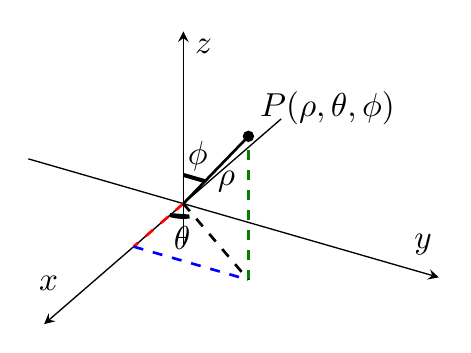
\begin{tikzpicture}[scale=1.2]
\begin{axis}[
    view={120}{30},
    axis equal,
    axis lines=middle,
    xlabel={$x$},ylabel={$y$},zlabel={$z$},
    grid=none,ticks=none,
    xmin=-0.5, xmax=3,
    ymin=-0.5, ymax=4,
    zmin=-1.5, zmax=6
]
\addplot3[Red,thick,dashed] coordinates {
    (0,0,0)
    (3,0,0)
};
\addplot3[Blue,thick,dashed] coordinates {
    (3,0,0)
    (3,4,0)
};
\addplot3[Green,thick,dashed] coordinates {
    (3,4,0)
    (3,4,5)
};
\addplot3[thick] coordinates {
    (0,0,0)
    (3,4,5)
};

\addplot3[only marks,mark=*,mark size=1.5pt]
    coordinates { (3,4,5) };
\addplot3[thick,dashed] coordinates {
    (0,0,0)
    (3,4,0)
};

\node at (3,4,5) [above right] {$P(\rho,\theta,\phi)$};
\addplot3[
    domain=0:43,
    samples=30,
    very thick,
    variable=\t
] (
    {0.8*cos(\t)},
    {0.8*sin(\t)},
    {0}
);
\node at (1.8,1,0) {$\theta$};
\addplot3[
    domain=0:0.75,
    samples=30,
    very thick,
    variable=\t
] (
    {0},
    {\t},
    {cos(pi*\t)}
);
\node at (0,0.5,1.8) {$\phi$};
\node at (0,1.5,1.2) {$\rho$};
\end{axis}
\end{tikzpicture}
\end{figure}

Using the figure above, we can define the spherical coordinate of
a point $P$.

\begin{definition}{}{}
Given a point $P$ with $\rho \geq 0$, $0 \leq \theta < 2\pi$, and
$0 \leq \phi \leq \pi$, the \textbf{spherical coordinate} of $P$
is $(\rho, \theta, \phi)$.
\end{definition}

Using this definition, let's take a look at how the spherical
coordinates can be converted to cylindrical and rectangular
coordinates. From the diagram, it is evident that the following
equations hold.
\[
r = \rho\sin\phi, \quad
x = \rho\sin\phi\cos\theta, \quad
y = \rho\sin\phi\sin\theta, \quad
z = \rho\cos\phi
\]
Similarly, the following equations holds for converting rectangular
coordinates to spherical coordinates.
\[
\rho = \sqrt{x^2 + y^2 + z^2}, \quad
\tan\theta = \frac{y}{x}, \quad
\phi = \cos^{-1} \left( \frac{z}{\sqrt{x^2 + y^2 + z^2}} \right)
\]
Just like the cylindrical coordinates, spherical coordinates can
help in representing certain surfaces. Consider the following
example.

\begin{problem}{}{}
Rewrite the hyperboloid $x^2 + y^2 - z^2 = 1$ using spherical
coordinates.
\end{problem}
\begin{solution}
First, notice that $\rho = \sqrt{x^2 + y^2 + z^2}$ and
$z = \rho\cos\phi$. Substituting, $\rho^2 - 2\rho^2\cos^2\phi = 1$
is obtained. Therefore, the hyperboloid can be written as
$\rho^2 = \frac{1}{1 - 2\cos^2\phi} = -\sec{2\phi}$.
\end{solution}

This is it for different coordinate representations of a point in
3-space! From our next notes, we will begin discussing about different
functions and derivatives.

\end{document}


